\documentclass[10pt]{beamer}
\usepackage{caption}
\usetheme{metropolis}
\usepackage{appendixnumberbeamer}
\usepackage{amsmath}
%
\setbeamercolor{frametitle}{bg=violet}
\setbeamerfont{caption}{size=\scriptsize}
\setbeamercolor{title separator}{fg=violet}
\setbeamercolor{progress bar in section page}{fg=violet}
\usepackage{outlines}
\usepackage{subfig}
\captionsetup[subfigure]{font=tiny,labelfont=tiny}
\setbeamerfont{footnote}{size=\tiny}


\title{Runtime Adaptivity through Splittable Tasks}
\subtitle{Ste||ar Group}
\author{Shahrzad Shirzad}
\date{July 7, 2020}
\institute{Louisiana State University}
%\titlegraphic{
\includegraphics[height=10mm]{logos/stellar_4x1.pdf}}
\titlegraphic{
	\begin{tikzpicture}[overlay, remember picture]
	\node[at=(current page.south east), anchor=south east] {%
		
\includegraphics[width=.25\textwidth]{logos/stellar_4x1.pdf} 
	};
	\node[at=(current page.south west), anchor=south west] {%
		
\includegraphics[width=.50\textwidth]{logos/LSU.png} 
	};
	\end{tikzpicture}
}


\begin{document}
\setbeamercolor{background canvas}{bg=white}


\maketitle

%\begin{frame}{Outline}
%  \setbeamertemplate{section in toc}[sections]
%  \tableofcontents[hideallsubsections]
%\end{frame}


\begin{frame}{Objective}
	\begin{outline}
		To provide a runtime adaptive solution to control task granularity. 
		\begin{columns}
				\column{0.45\linewidth}
			\begin{figure}
				\centering
				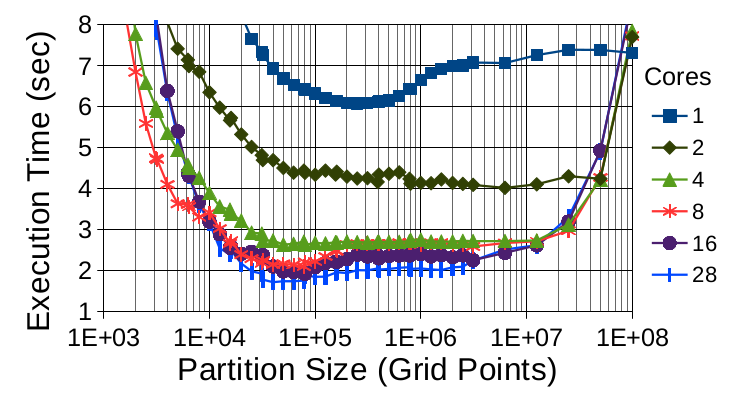
\includegraphics[scale=.22]{images/task_granularity.png}
				\caption{The effect of task size on execution time for Stencil application}			
			\end{figure}				
		\column{0.45\linewidth}
		\begin{figure}
			\centering
			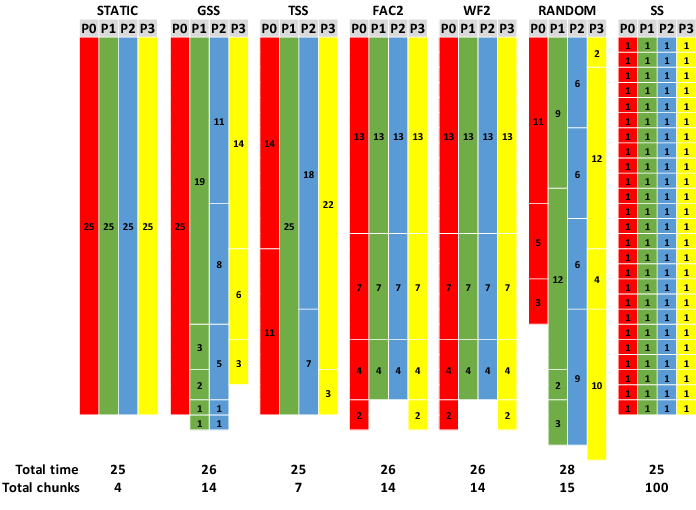
\includegraphics[width=0.8\linewidth]{images/loop_1.png}
			\caption{An example of effect of different loop scheduling methods}		
			\label{figloop}		
		\end{figure}
	\end{columns}
\footnote{Grubel, Patricia, et al. "The performance implication of task size for applications on the hpx runtime system." 2015 IEEE International Conference on Cluster Computing. IEEE, 2015.}
\footnote{Ciorba, Florina M., Christian Iwainsky, and Patrick Buder. "OpenMP loop scheduling revisited: making a case for more schedules." International Workshop on OpenMP. Springer, Cham, 2018.}
	\end{outline}		
\end{frame}



\begin{frame}{Splittable Tasks}
	\begin{outline}
		
		\1Splittable tasks are tasks that could be partitioned into smaller tasks, when sufficient parallelism is available.
		\2 A task could be splitted into two or more tasks, depending on the splitting strategy.
		
		\vspace{\baselineskip}
		\begin{figure}
			\centering
			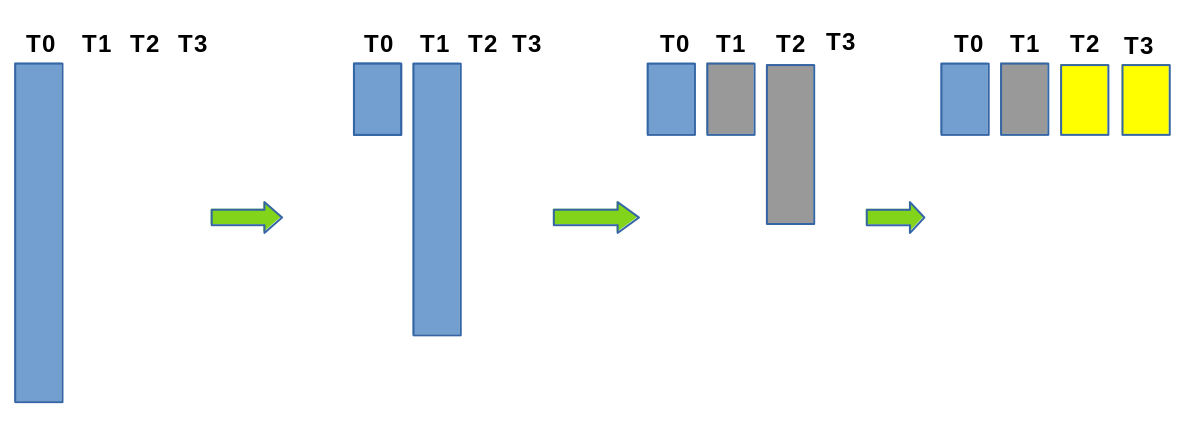
\includegraphics[width=0.72\linewidth]{images/spt_simple.png}
				\caption{A simple example of splittable tasks}
			
		\end{figure}
	\2Two modes: All, Idle\_mask
	\end{outline}
\end{frame}


\begin{frame}{Splittable Executor Modes: All}
	\begin{outline}
					
		\begin{columns}		
	\column{0.38\linewidth}
	{Splits the tasks into two parts, $\frac{1}{P}$ of the original task size remains for the current worker, the rest is assinged to the next available worker. $P$ is set to the number of cores and is decremented at each split.}
	\column{0.6\linewidth}  
\begin{figure}[]
	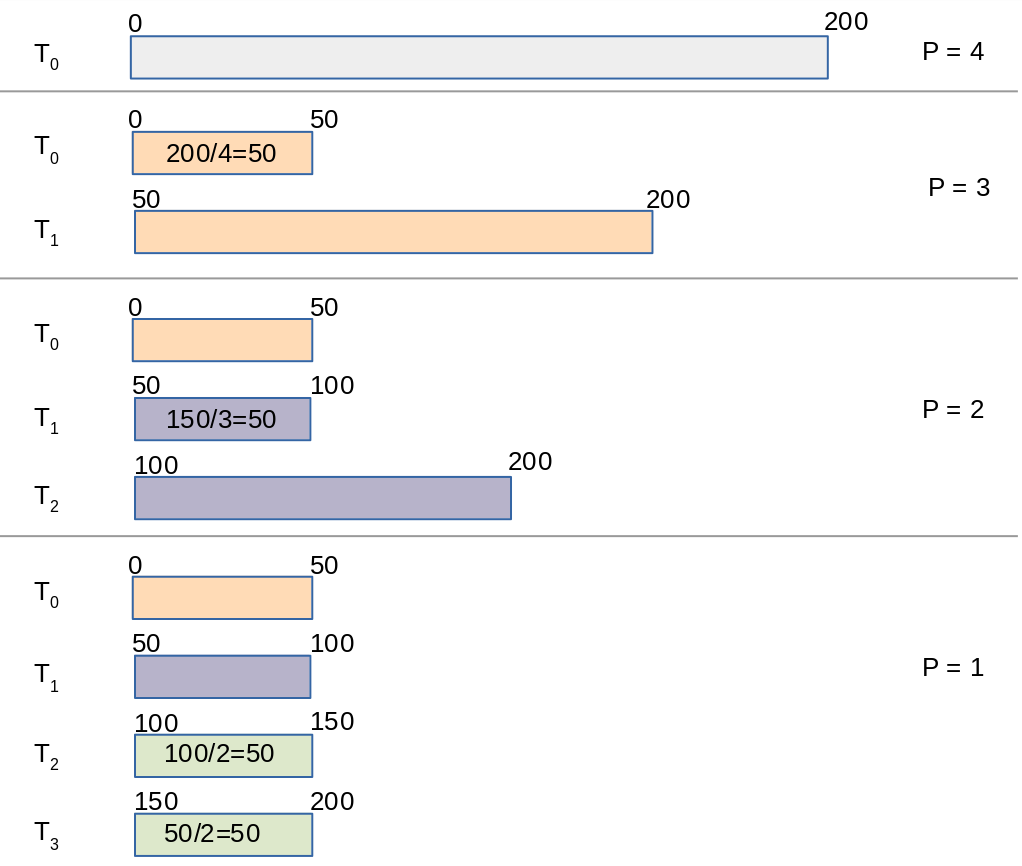
\includegraphics[width=0.98\linewidth]{images/spt_all.png}
	\caption{An example of loop scheduling using splittable tasks in "all" mode with 200 iterations, ran on 4 cores.}
	\end{figure}
		
	\end{columns}
			
		\end{outline}
	\end{frame}

	\begin{frame}{Splittable Executor Modes: Idle Mask}
		\begin{outline}
			\begin{columns}		
				\column{0.38\linewidth}
				{Task is equally splitted among the idle cores, and the generated tasks are explicitly assigned to the idle cores.}
				\column{0.6\linewidth}  
				\begin{figure}[]
					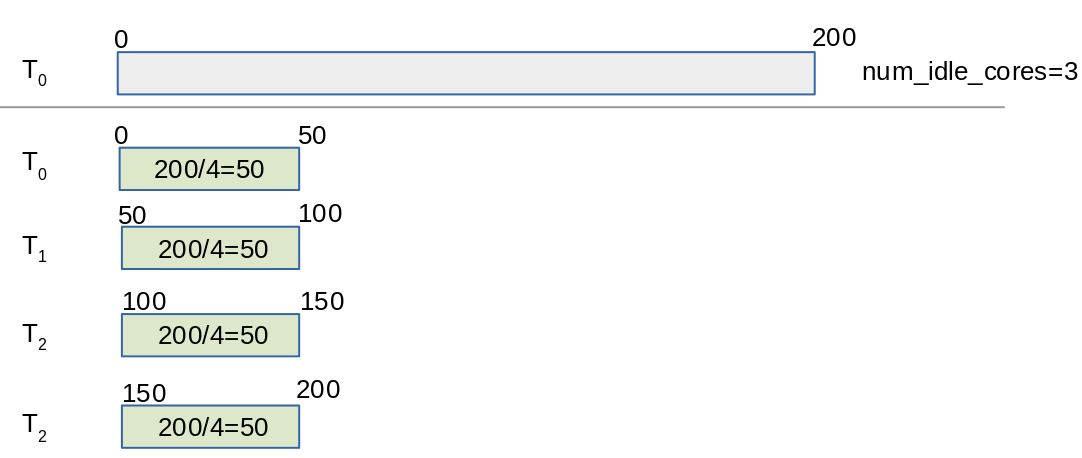
\includegraphics[width=0.99\linewidth]{images/spt_idle_mask.png}
					\caption{An example of loop scheduling using splittable tasks in "idle mask" mode with 200 iterations, ran on 4 cores.}
				\end{figure}				
			\end{columns}
		\end{outline}
	\end{frame}
	
	
	\begin{frame}{Results}
		\begin{outline}	
			\1Benchmark
			\2 HPX parallel for-loop with iteration length of $1{\mu}sec$
			\2 $ps = num\_{iterations}\times{iter\_{length}}=num\_{iterations}$
			\2 Run the benchmark on 1, 2,..,8 cores for diffrent problem sizes: 1000, 10000, 100000, 1000000, 10000000 
		\end{outline}
	\end{frame}
		
			\begin{frame}{Results}
			\begin{outline}	
				\begin{figure}[H]
					\centering
					\subfloat[]{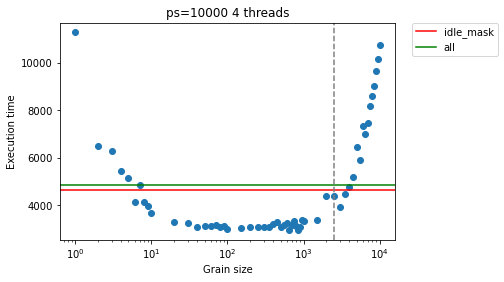
\includegraphics[scale=.3]{images/splittable/ps-th/marvin_10000_4.png}\label{fig10:a}}
					\subfloat[]{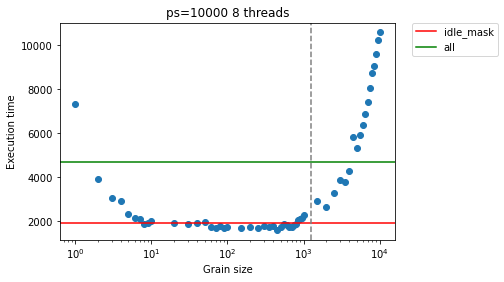
\includegraphics[scale=.3]{images/splittable/ps-th/marvin_10000_8.png}\label{fig10:b}}\hfill
					\subfloat[]{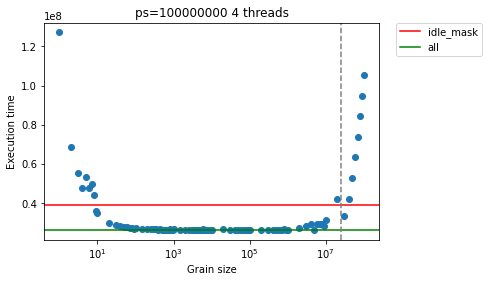
\includegraphics[scale=.3]{images/splittable/ps-th/marvin_100000000_4.png}\label{fig10:c}}
					\subfloat[]{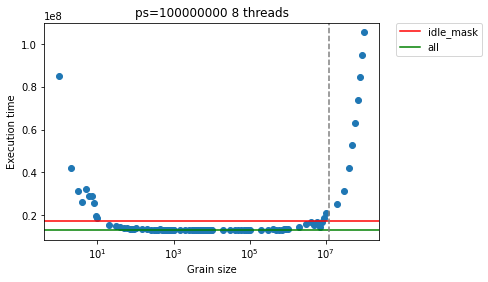
\includegraphics[scale=.3]{images/splittable/ps-th/marvin_100000000_8.png}\label{fig10:d}}		
					\caption{}
					\label{fig10}
				\end{figure}
			\end{outline}
		\end{frame}
	
	%\section{Future Work}
	\begin{frame}{Results}
		\begin{outline}	
			\begin{figure}[H]
			\centering
			\subfloat[]{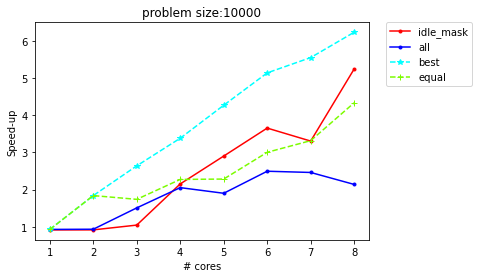
\includegraphics[scale=.3]{images/splittable/ps/marvin_old_10000.png}\label{fig10:a}}
			\subfloat[]{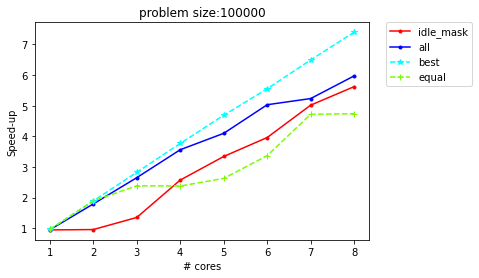
\includegraphics[scale=.3]{images/splittable/ps/marvin_old_100000.png}\label{fig10:b}}\hfill
			\subfloat[]{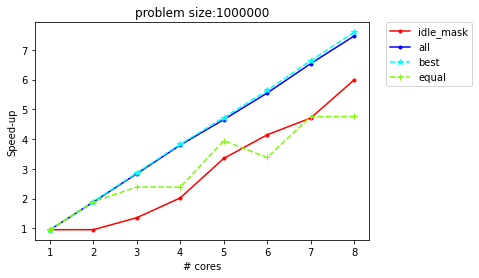
\includegraphics[scale=.3]{images/splittable/ps/marvin_old_1000000.png}\label{fig10:c}}
			\subfloat[]{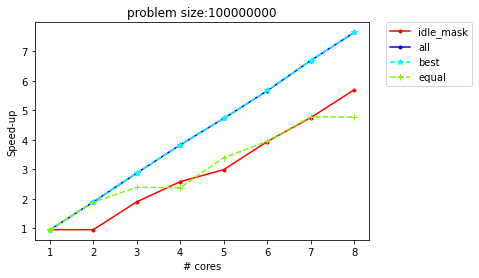
\includegraphics[scale=.3]{images/splittable/ps/marvin_old_100000000.png}\label{fig10:d}}\hfill
	
			\caption{}
			\label{fig10}
		\end{figure}
		\end{outline}
	\end{frame}

\begin{frame}[standout]
  Thank you!
\end{frame}

\begin{frame}{OTF2 Traces: all mode}
		\begin{figure}[]
		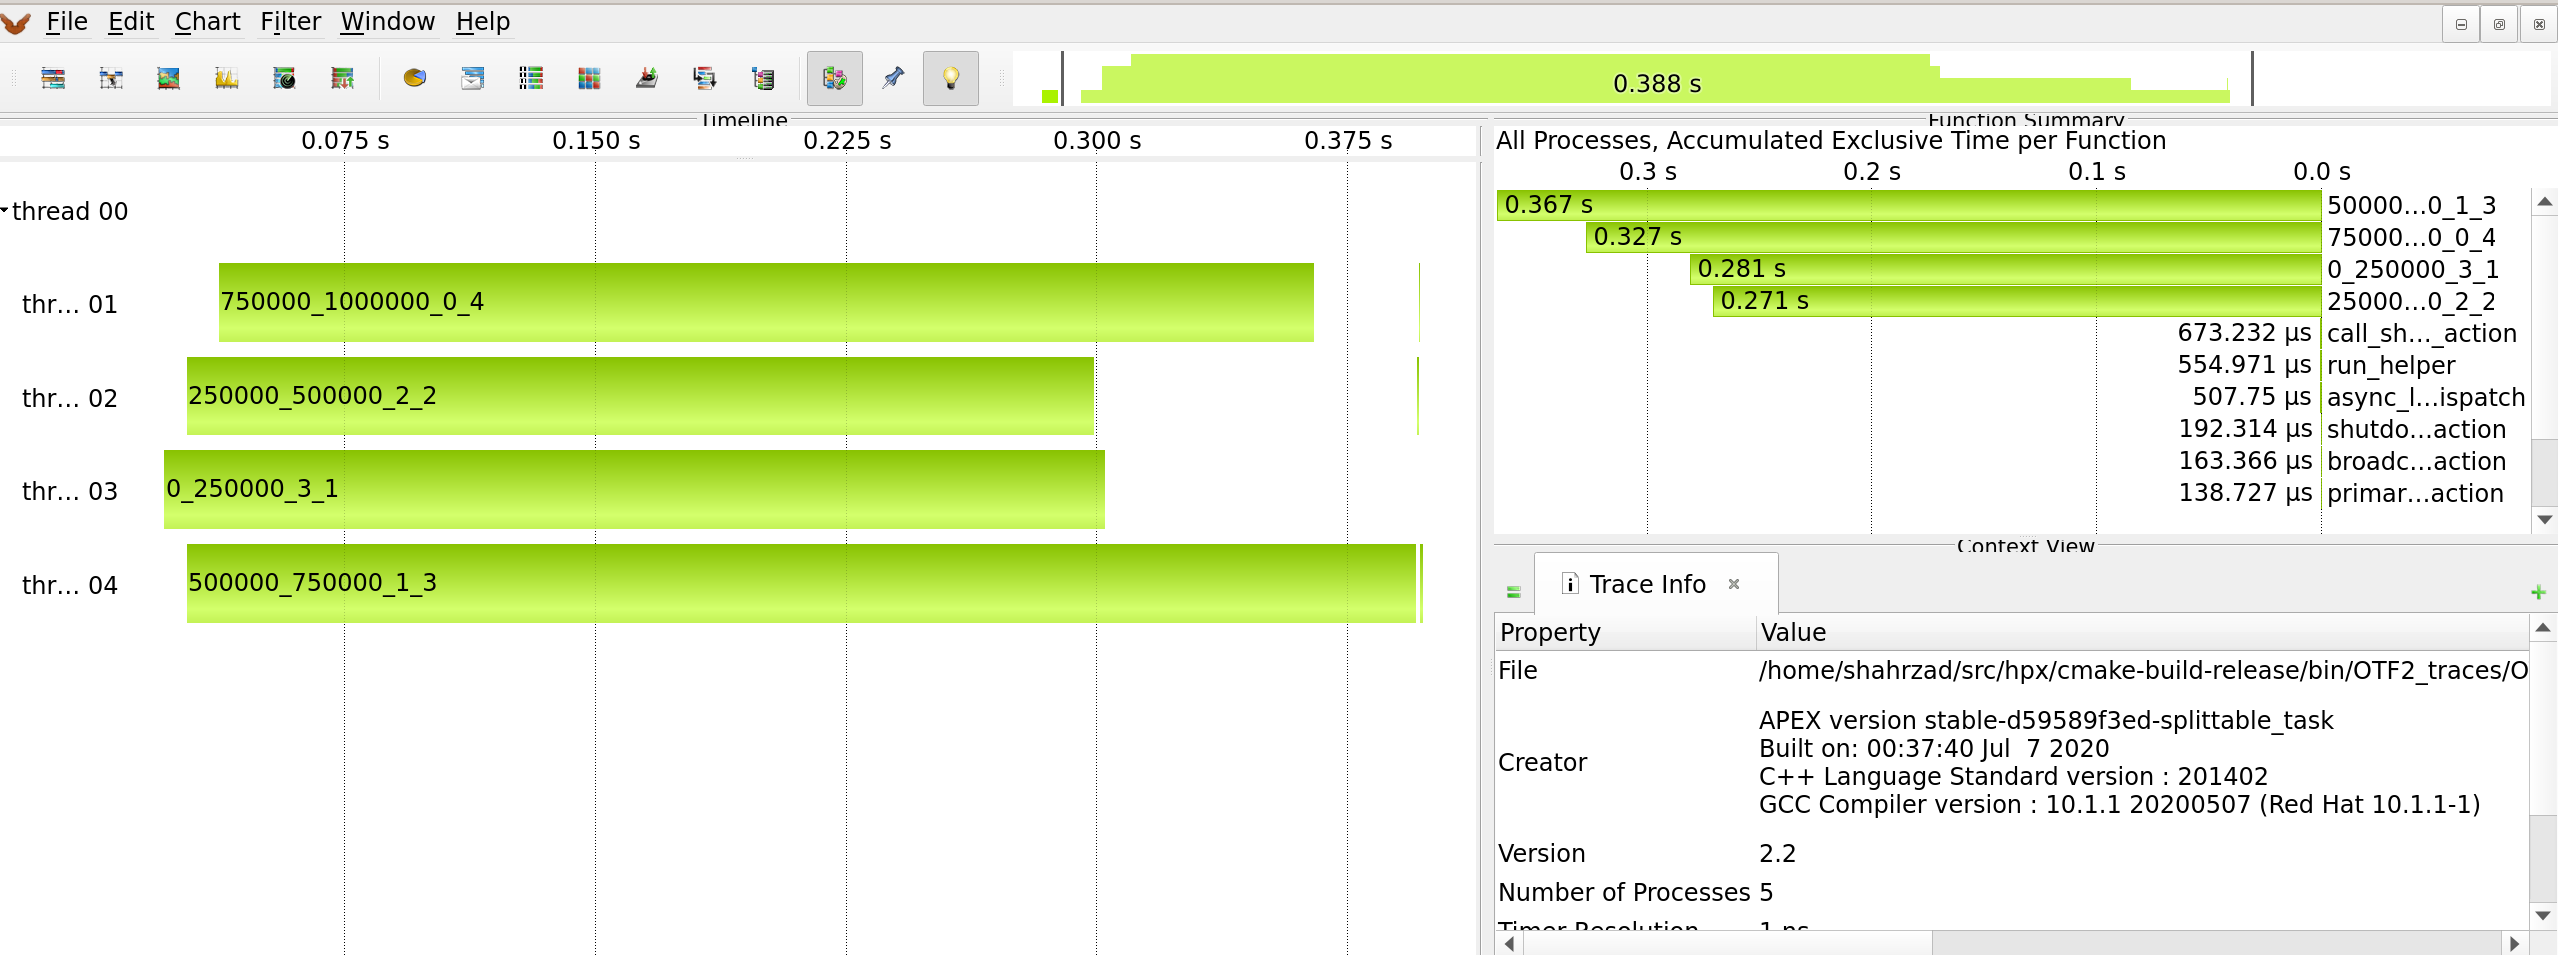
\includegraphics[width=0.99\linewidth]{images/splittable/traces/all_1000000_4.png}
		\caption{}
	\end{figure}	
\end{frame}

\begin{frame}{OTF2 Traces: idle mask mode}
	\begin{figure}[]
		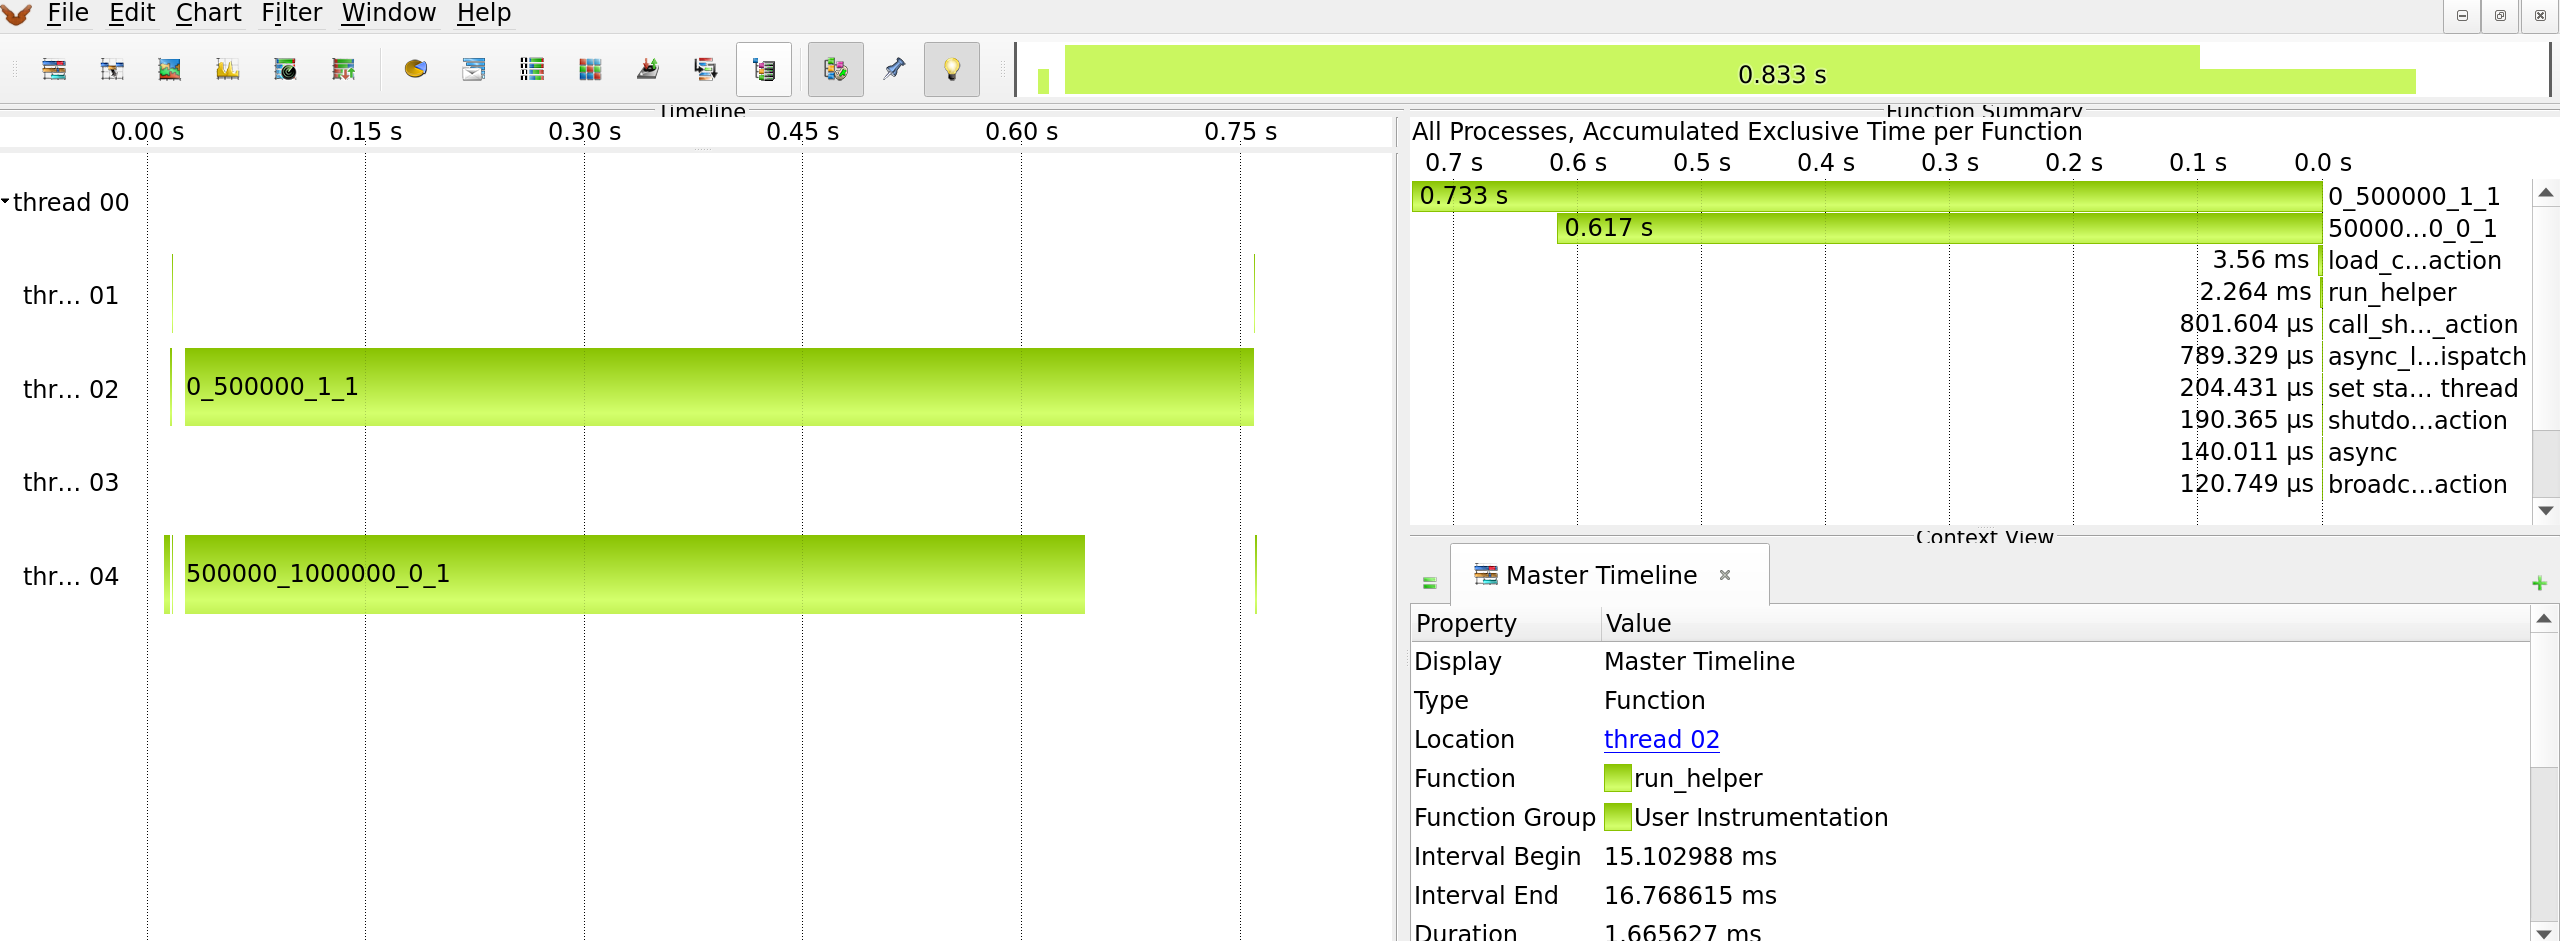
\includegraphics[width=0.99\linewidth]{images/splittable/traces/idle_mask_1000000_4.png}
		\caption{}
	\end{figure}	
\end{frame}
\end{document}